\documentclass[12pt]{article}

\usepackage[utf8x]{inputenc}
\usepackage[L7x, T2A]{fontenc}
\usepackage[lithuanian]{babel}
\usepackage{vwcol}  
\usepackage{sectsty}
\usepackage{setspace}
\usepackage{fancyhdr}
\usepackage{graphicx}
\usepackage{ragged2e}
\usepackage{titlesec}
\usepackage{epsfig}
\usepackage{indentfirst}
\usepackage[top=2cm, bottom=2cm, left=3cm, right=1.5cm]{geometry}

\usepackage{svg}

\makeatletter
\expandafter\let\csname L7x-cmd\endcsname\@changed@cmd
\makeatother

\addto\extraspolish{\fontencoding{L7x}\selectfont}
\addto\noextraspolish{\fontencoding{\encodingdefault}\selectfont}

\setlength\parindent{1cm}

\title{VILNIAUS UNIVERSITETAS \\
MATEMATIKOS IR INFORMATIKOS FAKULTETAS \\
PROGRAMŲ SISTEMŲ KATEDRA}
\author{}
\date{}

\pagestyle{fancy}
\fancyhead{}
\fancyfoot{}
\fancyfoot[R]{\thepage}
\renewcommand{\headrulewidth}{0pt}
\renewcommand{\baselinestretch}{1.5}

\begin{document}
	\clearpage
	\maketitle
	\thispagestyle{empty}

	\bigbreak
	\bigbreak
	\bigbreak
	\bigbreak

	\begin{center}
		\begin{Large}
			\textbf{Transporto priemonių skelbimų aplikacija} \\
		\end{Large}
		\begin{large}
			\textbf{Application for Vehicle Advertisement} \\
		\end{large}
		Programų sistemų inžinerijos I laboratorinis darbas Nr. 1 \\

		\bigbreak
		\bigbreak
		\bigbreak
		\bigbreak
		\bigbreak
		\bigbreak
		\bigbreak
		\bigbreak
		\bigbreak

		\begin{tabular}{ll}
			Atliko:        & 2 kurso 5 grupės studentai \\
		               	   & Toma Burneikaitė \\
		               	   & Žygimantas Stongvilas \\
		                   & Mantas Jurčius \\
		                   & Rimvydas Meškauskas \\
			Darbo vadovas: & asist., dr., Vytautas Valaitis
		\end{tabular}

		\bigbreak
		\bigbreak
		\bigbreak
		\bigbreak
		\bigbreak
		\bigbreak
		\bigbreak
		\bigbreak
		\bigbreak

		Vilnius - 2018
	\end{center}
	\pagebreak
	
	\section*{Anotacija}
	\addcontentsline{toc}{section}{Anotacija}
	\begin{indent}
	Dokumentas parengtas kaip programų sistemos inžinerijos dalyko laboratorinis darbas\\Nr. 1, kuriame pateikiamas suprojektuotos sistemos aprašymas. Programų sistemos architektūra apibrėžiama naudojantis 4+1 architektūros pjūvių modelį.
	\end{indent}
	\pagebreak

	{\setstretch{1.0}\tableofcontents}
	\pagebreak

	\section*{Įvadas}
	\addcontentsline{toc}{section}{Įvadas}
	
	\begin{indent}
	Šiame projektiniame darbe pristatomas automobilių skelbimų programėlės „AutoINF“ įgyvendinimas. Šio projekto vizija yra sukurti mobiliesiems įrenginiams skirtą programėlę, kuri leistų pasiekti automobilių skelbimus iš visos Europos. Idėja kilo iš to, kad dabar įvairių automobilių skelbimai yra daugybėje skirtingų puslapių (šaltinių) ir norint susirasti sau naudin-giausią pasiūlymą dažniausiai reikia pereiti per daugiau nei vieną puslapį. „AutoINF“ projekto tikslas yra sukurti programėlę, kuri supaprastintų automobilių ieškojimo procesą ir padėtų vartotojui sutaupyti laiko tą darant, surinkdama visus skelbimus iš populiariausių Europos automobilių skelbimų puslapių pagal vartotojo nurodytus kriterijus. Taip pat norima, kad programėle būtų paprasta naudotis ir kad šita programėlė sugebėtų pateikti kuo daugiau vartotojui aktualios informacijos apie tai, ko jis ieško.
	\end{indent}
	
%	\begin{flushleft}
%		\bigbreak\textbf{Programų sistemos pavadinimas}
%	\end{flushleft}
	
%	Pilnas programų sistemos pavadinimas – automobilių skelbimų aplikacija „AutoInf“ \\
	
%	\begin{flushleft}
%		\textbf{Dalykinė sritis}
%	\end{flushleft}	
	
%	Automobilių skelbimų iš visos Europos pateiktis vartotojams  \\
	
%	\begin{flushleft}
%		\textbf{Probleminė sritis}
%	\end{flushleft}
	
%	Užsienyje galima rasti pigesnių automobilių \\
	
%	\begin{flushleft}
%		\textbf{Naudotojai} 
%	\end{flushleft}
	
%	Žmonės, ieškantys automobilių \\
	
%	\begin{flushleft}
%		\textbf{Darbo pagrindas}
%	\end{flushleft}
	
%	Dokumentas parengtas kaip programų sistemos inžinerijos dalyko laboratorinis darbas\\Nr. 1, kuriame pateikiamas suprojektuotos sistemos aprašymas.
	\pagebreak

	\section{Užduotys ir jų vykdymo scenarijai}
	Šiame skyriuje pavaizduotos ir aprašytos sistemos vartotojų užduotys bei jų vykdymo scenarijai.
	\subsection{Sistemos vykdomos užduotys}
	Žemiau esančiame \ref{UseCase} paveikslėlyje pavaizduoti tikslai, kurių siekia sistema besinaudojantys agentai - automobilių ieškantys vartotojai bei sistemos administratoriai. Į sistemą žiūrima kaip į vieną visumą, neatskleidžiant jos implementacijos detalių.
	
	\begin{figure}[h]
		\begin{center}
			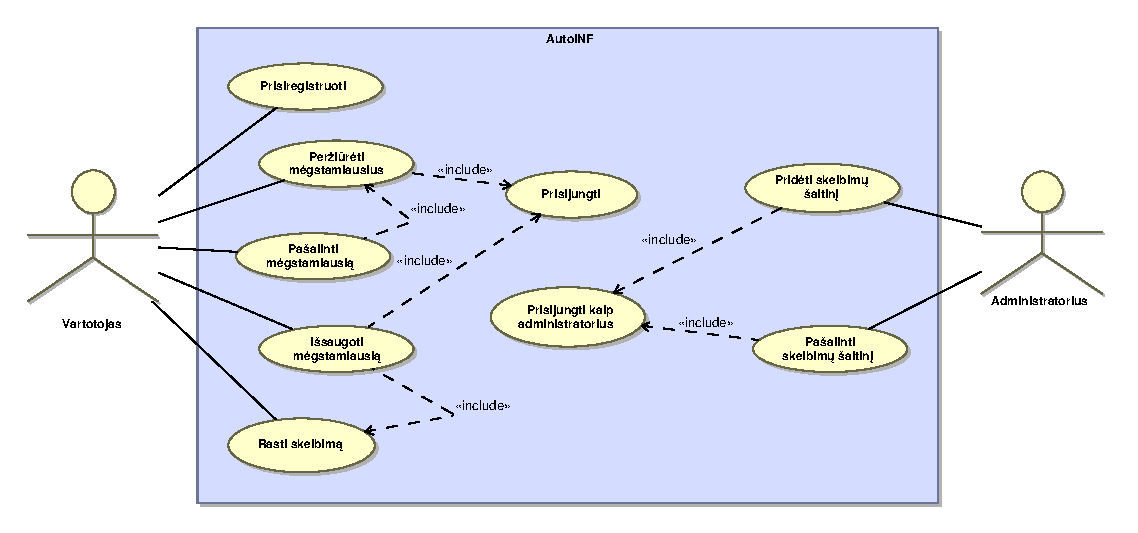
\includegraphics[width=\textwidth]{Tikslai.eps}
			\caption{Sistemos užduočių diagrama\label{UseCase}}
		\end{center}
	\end{figure}
	
	%\ref{UseCase} paveikslėlyje yra pavaizduoti tikslai, kurių siekia sistema besinaudojantys agentai - vartotojas ir administratorius
	\pagebreak

	\ref{UseCaseUser} paveikslėlyje pateiktos vartotojui prieinamos „AutoINF“ funkcijos: registracija, prisijungimas, peržiūrėti mėgstamiausius, pašalinti mėgstamiausią, išsaugoti mėgstamiausią, rasti skelbimą. Daugiau informacijos apie šias funkcijas yra tolimesnėse (\ref{RegisterSeq} - \ref{ViewFavSeq} pav.) sekų diagramose.
	
	\begin{figure}[h]
		\begin{center}
			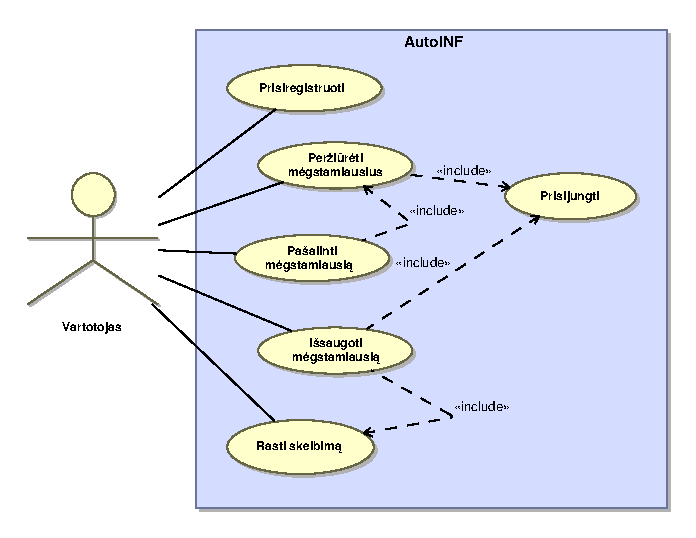
\includegraphics[width=0.7\textwidth]{TikslaiVartotojas.eps}
			\caption{Sistemos užduočių diagrama iš vartotojo perspektyvos\label{UseCaseUser}}
		\end{center}
	\end{figure}
	
%	\ref{UseCaseUser} paveikslėlyje pateiktos vartotojui prieinamos „AutoINF“ funkcijos: registracija, prisijungimas, peržiūrėti mėgstamiausius, pašalinti mėgstamiausius, išsaugoti mėgstamiausius, rasti skelbimą. Plačiau apie šias funkcijas rašoma tolimesnėse sekų diagramose.
	\pagebreak	
	
	\ref{UseCaseAdmin} paveikslėlyje pateiktos administratoriui prieinamos „AutoINF“ funkcijos: pridėti skelbimų šaltinį, pašalinti skelbimų šaltinį, pašalinti vartotojo paskyrą. Šios funkcijos labiau išplėtojamos tolimesnėje (\ref{ManSouSeq} pav.) sekų diagramoje. Administratorius prisijungia taip pat, kaip ir vartotojas, tik jam suteiktos administratoriaus teisės.	
	
	\begin{figure}[h]
		\begin{center}
			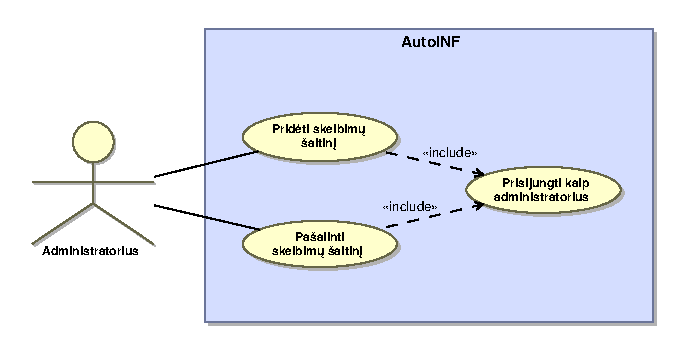
\includegraphics[width=0.7\textwidth]{TikslaiAdministratorius.eps}
			\caption{Sistemos užduočių diagrama iš administratoriaus perspektyvos\label{UseCaseAdmin}}
		\end{center}
	\end{figure}	
	
	\pagebreak
	
	\subsection{Užduoties „Prisiregistruoti“ įgyvendinimas}
	
	Vartotojo registracijos sistemoje užduoties vykdymas pavaizduotas \ref{RegisterSeq} paveikslėlyje. Vartotojas, atidaręs registracijos langą, turi suvesti prisiregistravimo duomenis. Paspaudus registracijos mygtuką, aplikacija patikrina, ar duomenys suvesti reikiamu formatu. Jei formatas teisingas, tai duomenys išsaugomi duomenų bazėje. Tada vartotojas yra infomuojamas apie sėkmingą registraciją ir yra prijungiamas prie sistemos.	
	
	\begin{figure}[h]
		\begin{center}
			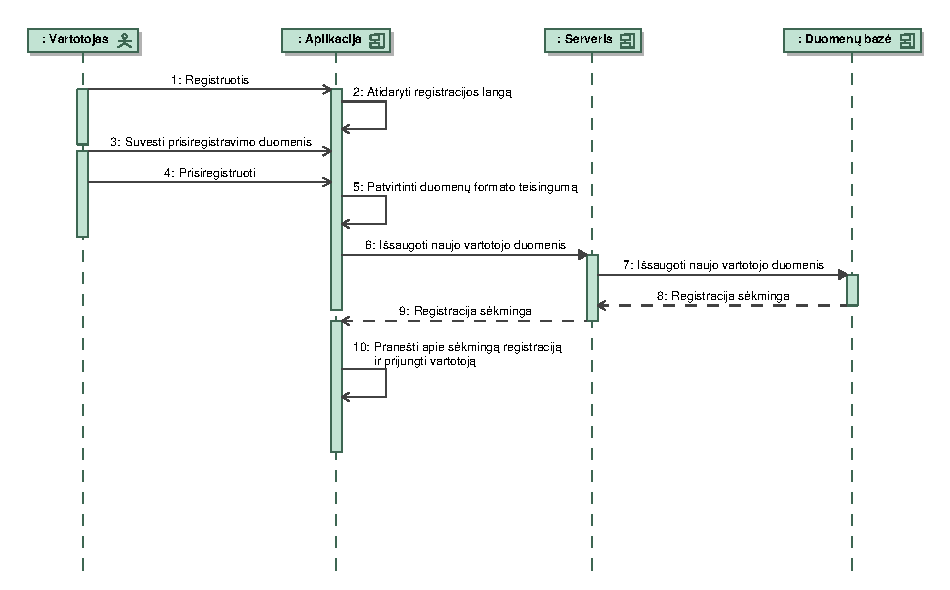
\includegraphics[width=\textwidth]{Prisiregistruoti.eps}
			\caption{Užduoties „Prisiregistruoti“ sekų diagrama\label{RegisterSeq}}
		\end{center}
	\end{figure}
	
	\pagebreak
	
	\subsection{Užduoties „Prisijungti“ įgyvendinimas}
	Vartotojo prisijungimo sistemoje užduoties vykdymas pavaizduotas \ref{LogInSeq} paveikslėlyje. Vartotojas, atidaręs prisijungimo langą, turi suvesti prisijungimo duomenis ir tada paspaudus prisijungimo mygtuką, duomenų bazėje yra patikrinama, ar toks vartotojas egzistuoja. Vartotojui prisijungus atsidaro pagrindinis langas, kuriame atsiranda funkcijos, prieinamos tik registruotiems vartotojams.
	\begin{figure}[h]
		\begin{center}
			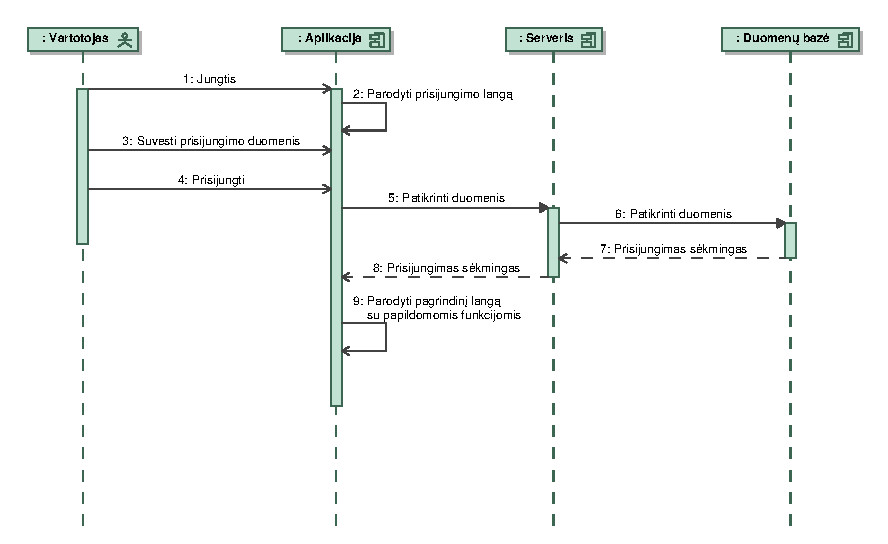
\includegraphics[width=\textwidth]{Prisijungti.eps}
			\caption{Užduoties „Prisijungti“ sekų diagrama\label{LogInSeq}}
		\end{center}
	\end{figure}
	

	\pagebreak
	
	\subsection{Užduoties „Rasti skelbimą“ įgyvendinimas}
	Skelbimų ieškojimo sistemoje užduoties vykdymas pavaizduotas \ref{FindAdvertSeq} paveikslėlyje. Vartotojas nebūtinai turi būti prisijungęs, kad galėtų pasinaudoti šia sistemos funkcija. Pirmiausia vartotojas turi pagrindiniame lange įvesti paieškos kriterijus (kai kurie filtrai yra privalomi). Paspaudus paieškos mygtuką, sistema suranda filtrą atitinkančius skelbimus ir juos parodo. Vartotojui paspaudus ant skelbimo atsidaro skelbimo langas.
	\begin{figure}[h]
		\begin{center}
			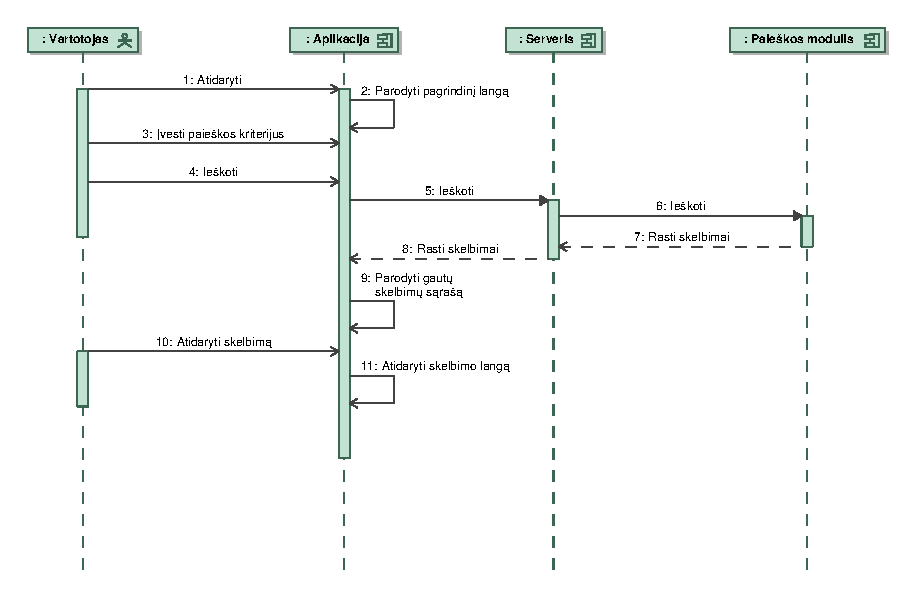
\includegraphics[width=\textwidth]{RastiSkelbima.eps}
			\caption{Užduoties „Rasti skelbimą“ sekų diagrama\label{FindAdvertSeq}}
		\end{center}
	\end{figure}
	
	
	\pagebreak
	
	\subsection{Užduoties „Išsaugoti mėgstamiausią“ įgyvendinimas}
	Mėgstamo skelbimo išsaugojimo užduoties vykdymas pavaizduotas \ref{SaveFavSeq} paveikslėlyje. Ši funkcija yra pasiekiama tada ir tik tada, kai vartotojas yra prisijungęs prie sistemos. Norėdamas išsaugoti skelbimą, vartotojas pirmiausia turi susirasti skelbimą ir tada  paspausti šio skelbimo išsaugojimo mygtuką. Apie sėkmingą skelbimo išsaugojimą vartotojas yra informuojamas.
	\begin{figure}[h]
		\begin{center}
			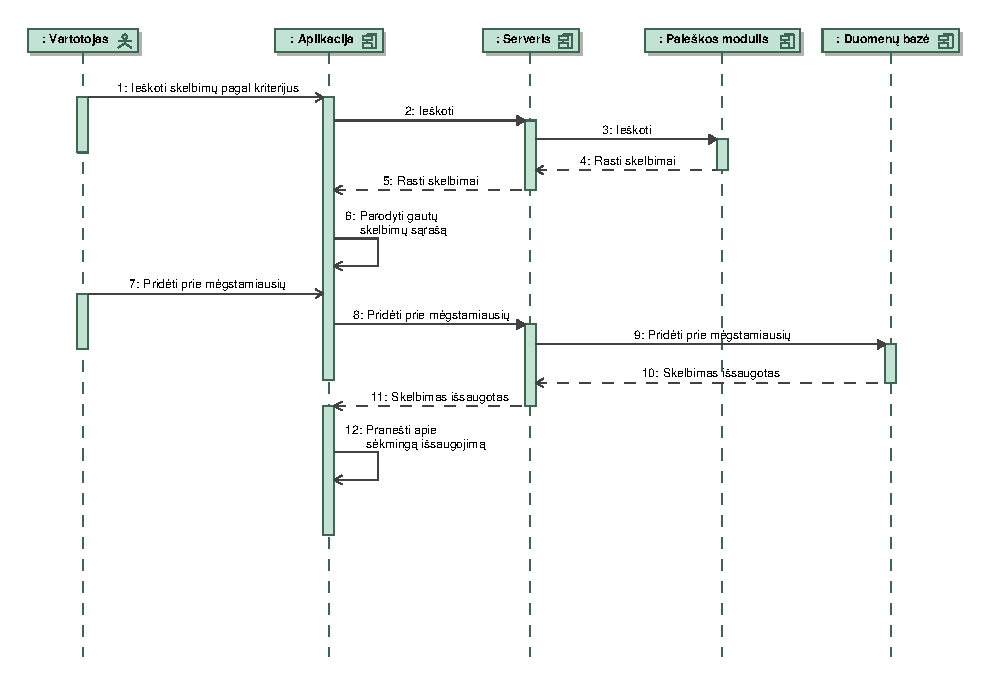
\includegraphics[width=\textwidth]{IssaugotiMegstamiausia.eps}
			\caption{Užduoties „Išsaugoti mėgstamiausią“ sekų diagrama\label{SaveFavSeq}}
		\end{center}
	\end{figure}
	
	
	\pagebreak
	
	\subsection{Užduoties „Pašalinti mėgstamiausią“ įgyvendinimas}
	Mėgstamo skelbimo pašalinimo užduoties vykdymas  pavaizduotas \ref{DelFavSeq} paveikslėlyje. Ši funkcija yra pasiekiama tada ir tik tada, kai vartotojas yra prisijungęs prie sistemos bei yra išsaugojęs bent vieną mėgstamą skelbimą. Pirmiausia vartotojas atsidaro mėgstamiausių skelbimų sąrašą. Tada pasirenka, kurį skelbimą jis nori pašalinti, ir paspaudžia pašalinimo mygtuką. Sėkmingai pašalinus skelbimą iš sąrašo, šis sąrašas yra atnaujinamas.
	\begin{figure}[h]
		\begin{center}
			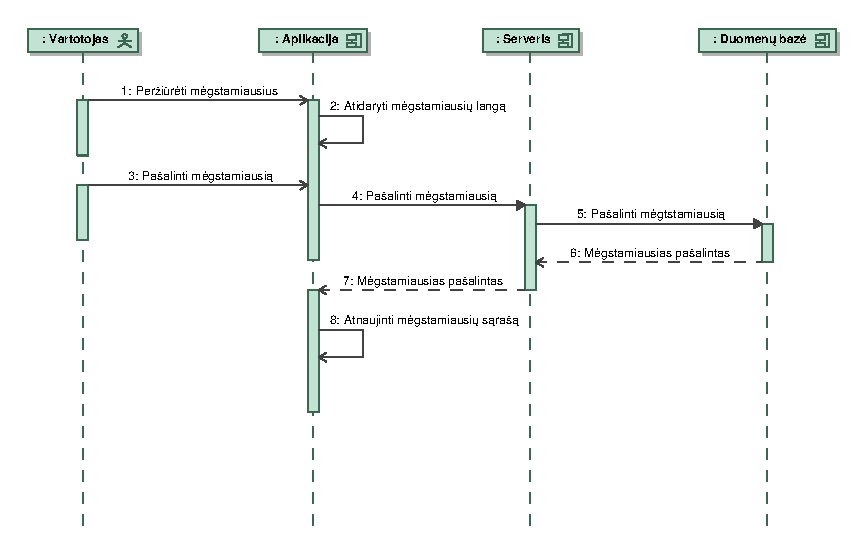
\includegraphics[width=\textwidth]{PasalintiMegstamiausia.eps}
			\caption{Užduoties „Pašalinti mėgstamiausią“ sekų diagrama\label{DelFavSeq}}
		\end{center}
	\end{figure}
	
	\pagebreak
	
	\subsection{Užduoties „Peržiūrėti mėgstamiausius“ įgyvendinimas}
	Mėgstamiausių skelbimų peržiūrėjimo užduoties vykdymas pavaizduotas \ref{ViewFavSeq} paveikslėlyje. Ši funkcijas pasiekiama tada ir tik tada, kai vartotojas yra prisijungęs prie sistemos. Vartotojui pasirinkus mėgstamiausių skelbimų langą, sistema parodo šio vartotojo mėgstamiausių skelbimų sarašą.
	\begin{figure}[h]
		\begin{center}
			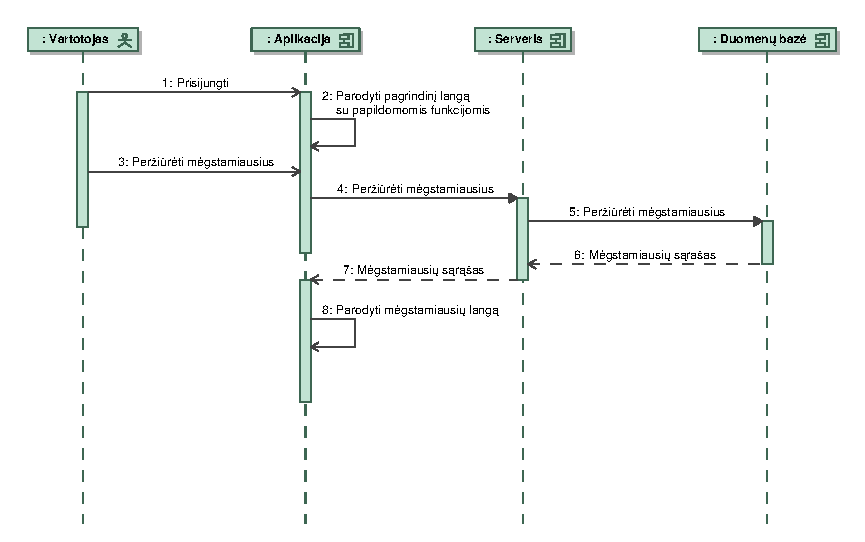
\includegraphics[width=\textwidth]{PerziuretiMegstamiausius.eps}
			\caption{Užduoties „Peržiūrėti mėgstamiausius“ sekų diagrama\label{ViewFavSeq}}
		\end{center}
	\end{figure}
	
	\pagebreak
	
	\subsection{Užduoties „Tvarkyti skelbimų šaltinius“ įgyvendinimas}
	Skelbimų šaltinių tvarkymo užduoties vykdymas yra pavaizduotas \ref{ManSouSeq} paveikslėlyje. Šia funkcija gali pasinaudoti tik administratorius. Administratorius, atsidaręs skalbimų šaltinių langą, gali pasirinkti, ką jis nori su šaltiniais daryti: pridėti naują skelbimų šaltinį ar pašalinti jau pridėtą šaltinį. Norėdamas pridėti šaltinį, administratorius spaudžia mygtuką, skirtą naujam šaltiniui pridėti, o siekdamas pašalinti skelbimą, administratorius turi pasirinkti šaltinį iš šaltinių sąrašo ir pasirinkti šaltinio pašalinimą. Tiek po šaltinio pridėjimo, tiek po šaltinio pašalinimo skelbimų šaltinių sąrašas yra atnaujinamas.
	\begin{figure}[h]
		\begin{center}
			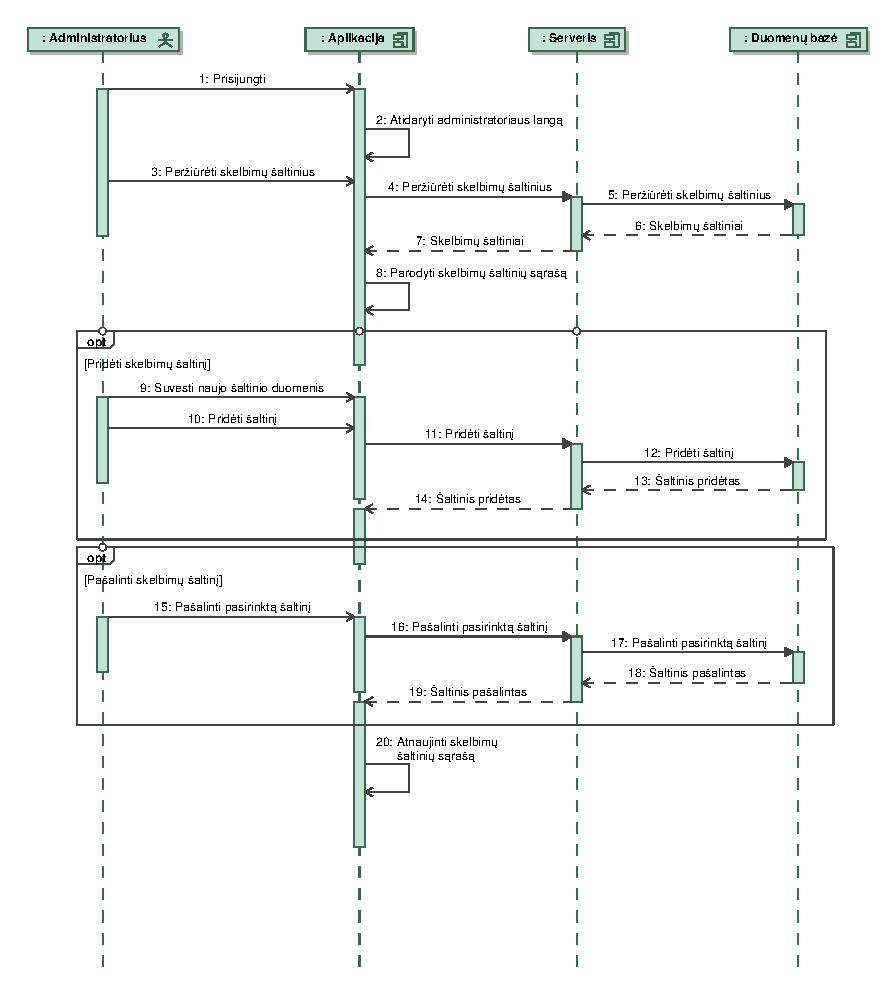
\includegraphics[width=0.8\textwidth]{TvarkytiSkelbimuSaltinius.eps}
			\caption{Užduoties „Tvarkyti skelbimų šaltinius“ sekų diagrama\label{ManSouSeq}}
		\end{center}
	\end{figure}

	\pagebreak
	
	\section{Struktūrinis programų sistemos modelis}
	Šiame skyriuje yra pateikta sistemos klasių diagrama ir, pasitelkiant objektų diagramą, parodytas sistemos naudojimo pavyzdys.
	\subsection{Klasių diagrama}
	
	Žemiau pateiktame \ref{ClassDiagram} paveikslėlyje yra išskirtos pagrindinės esybės, kurios yra naudojamos sistemoje. Klases siejantys ryšiai pasižymi kardinalumu. Kitaip sakant, nustatytas konkretus ryšių skaičius ar skaičių aibė, kurios turės klasės egzempliorius su tam tikros kitos klasės egzemplioriais.
	
	\begin{figure}[h]
		\begin{center}
			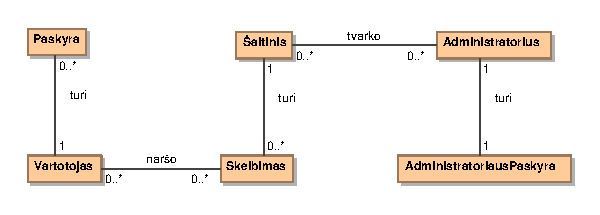
\includegraphics[width=\textwidth]{KlasiuDiagrama.eps}
			\caption{Klasių diagrama\label{ClassDiagram}}
		\end{center}
	\end{figure}
	
	Šioje sistemoje egzistuoja dviejų rūšių paskyros: paprasta paskyra ir administratoriaus paskyra. Paprastas vartotojas gali turėti daug paskyrų (pvz.: pamiršta visus duomenis apie savo paskyrą, tai jis gali susikurti naują), o viena paskyra priklauso tik vienam vartotojui. Administratorius gali turėti tik vieną paskyrą: vartotojui, kuriam suteikiamos administratoriaus teisės, išduodamas vienkartinis kodas, kurį įvedus sukuriama speciali administratoriaus paskyra. Administratorius tvarko šaltinius (t.y. prideda arba pašalina šaltinius). Kiekvienas šaltinis gali būti tvarkomas kelių arministratorių ir taip pat kiekvienas administratorius gali tvarkyti kelis šaltinius. Vartotojai gali naršyti daug skelbimų ir visi kelbimai gali būti naršomi kelių vartotojų. Visi skelbimai yra paimti iš kokių nors šaltinių. Kiekvienas skelbimas gali būti paimtas tik iš vieno šaltinio, tačiau kiekvienas šaltiniai gali turėti daug skelbimų.
	\pagebreak
	
	\subsection{Objektų diagrama}
	
	Šiame skyrelyje esančios objektų diagramos iš esmės patvirtina anksčiau pateiktą klasių diagramą. Taip pat pateikia tipinį pavyzdžį, kaip klasės bus naudojamos sistemoje.
	
	\begin{figure}[h]
		\begin{center}
			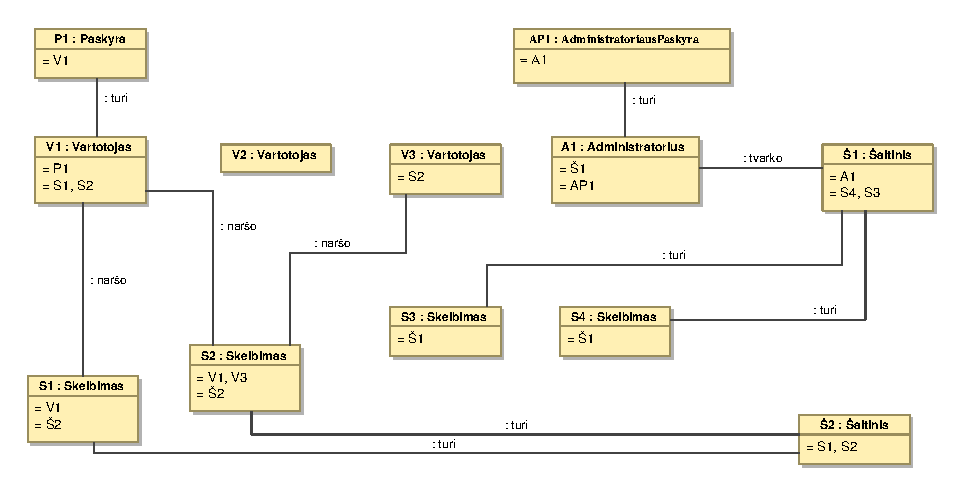
\includegraphics[width=\textwidth]{ObjektuDiagrama.eps}
			\caption{Objektų diagrama\label{ObjectDiagram}}
		\end{center}
	\end{figure}
	
	Aukščiau esančiame \ref{ObjectDiagram} paveikslėlyje parodyta tipinė sistemos situacija, kai yra sukurtos dvi paskyros: viena yra vartotojo, kita - administratoriaus. Taip pat yra dar du vartotojai, iš kurių vienas tuo momentu nieko nedaro sistemoje, kol kitas kartu su registruotu vartotoju naršo skelbimus (keli vartotojai gali naršyti tą patį skelbimą vienu metu). Taip pat yra keturi skelbimai, ir visi priklauso kažkuriam vienam šaltiniui, kol šaltiniai turi daugiau nei po vieną skelbimą (šaltiniai gali ir neturėti skelbimų). Taip pat iš diagramos galima matyti, kad administratorius gali tvarkyti šaltinius.
	\pagebreak
	
	\section{Programų sistemos komponentai}
	
	Šiame skyriuje yra pavaizduoti sistemos komponentai. Sistemos komponentų dekompozicija įgyvendinta „top-down“ būdu.	
	
	\subsection{Konteksto diagrama}
	Abstrakčiausias (aukščiausias) komponentų struktūros lygis parodomas \ref{Components1} paveikslėlyje.
	\begin{figure}[h]
		\begin{center}
			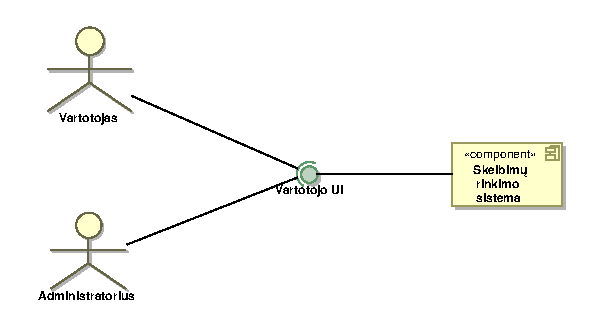
\includegraphics[width=\textwidth]{Komponentai1.eps}
			\caption{Konteksto komponentų diagrama\label{Components1}}
		\end{center}
	\end{figure}
	
	 Visa sistema laikoma kaip vienas darinys ir parodoma sąsaja su išore:
	
	\begin{itemize}	
		\item Interfeisai, kuriais išoriniai vartotojai naudojasi visa sistema
		\item Išorinių sistemų interfesiai, kuriais naudojasi sistema
	\end{itemize}
	
	Tiek vartotojas, tiek administratorius turi naudotis tuo pačiu vartotojo UI interfeisu. To priežastis yra ta, kad abu vartotojai naudojasi ta pačia sistema, tik su šiek tiek skirtingomis galimybėmis.	
	\pagebreak

	\subsection{Skelbimų rinkimo sistemos dekompozicija}
	Žemiau esančiame \ref{Components2} paveikslėlyje detalizuojamas \ref{Components1} paveikslėlyje esantis „Skelbimų rinkimo sistema“ komponentas.
	\begin{figure}[h]
		\begin{center}
			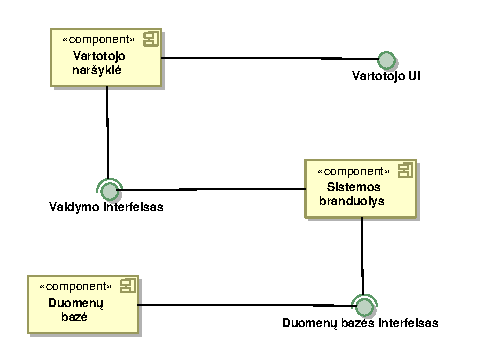
\includegraphics[width=0.9\textwidth]{Komponentai2.eps}
			\caption{Skelbimų rinkimo sistemos komponento dekompozicija\label{Components2}}
		\end{center}
	\end{figure}

	\textbf{Vartotojo naršyklė} - komponentas, sukuriantis vartotojo interfeisą bei vykdantis komuni-kaciją tarp vartotojo ir sistemos branduolio.

	
	\textbf{Sistemos branduolys} - komponentas, priimantis prašymus iš vartotojo naršyklės, kontroliuojantis duomenų gavimą ar išsaugojimą duomenų bazėje bei siunčiantis duomenis vartotojo naršyklei.

	
	\textbf{Duomenų bazė} - komponentas, kuriame saugoma informacija apie registruotus vartotojus ir kartu tos paskyros mėgstamiausius skelbimus.
	\pagebreak

	\subsection{Sistemos branduolio dekompozicija}
	\ref{Components3} paveikslėlyje smulkinamas \ref{Components2} paveikslėlyje esantis „Sistemos branduolio“ komponentas.
	\begin{figure}[h]
		\begin{center}
			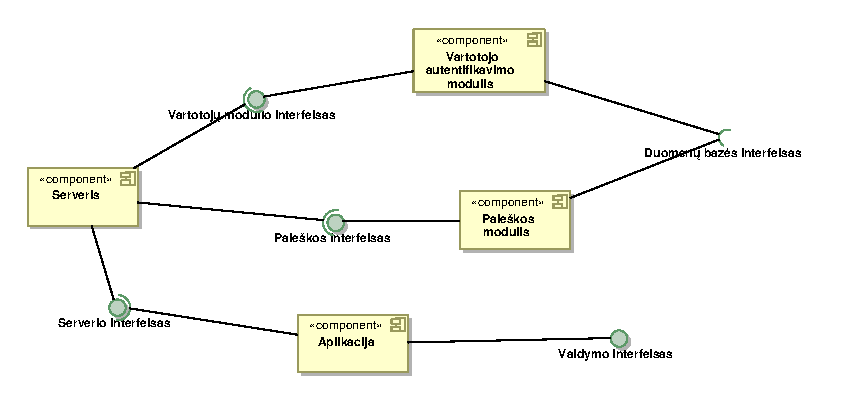
\includegraphics[width=\textwidth]{Komponentai3.eps}
			\caption{Sistemos branduolio komponento dekompozicija\label{Components3}}
		\end{center}
	\end{figure}

	 \bigbreak Jį sudarantys komponentai:\bigbreak
	
	\textbf{Vartotojo autentifikavimo modulis} - šis komponentas vykdo vartotojų autetifikaciją. Jo funkcijos: vartotojų registravimas, prisijungimas.
	
	\textbf{Paieškos modulis} - komponentas, pagal tam tikrus nurodytus kriterijus surandantis skelbimus.
	
	\textbf{Serveris} - komponentas, valdantis prieigą prie duomenų.
	
	\textbf{Aplikacija} - komponentas, kuris pateikia vartotojui skelbimų sąrašą, konkrečių skelbimų detalesnę informaciją.
	\pagebreak

	\section{Dinaminis programų sistemos modelis}
	Šiame skyriuje parodota, kaip vyksta šios sistemos veiksmai bei aprašytos kai kurios galimos vartotojų užduotys. 
	
	\subsection{Vartotojo registracijos veiklos diagrama}
	Procesai, vykstantys vartotojo registracijos metu, parodyti \ref{RegisterActivity} paveikslėlyje. Registravimas vyksta tada, kai vartotojas įsijungia aplikaciją ir pasirenka „Registracija“. Tada vartotojui suvedus reikiamus duomenis sistema patikrina, ar viskas užpildyta teisingai. Jei ne, vartotojas gali bandyti vesti informaciją iš naujo arba išeiti iš registravimosi lango. Jei informacija užpildyta teisingai, vartotojas gali toliau naudotis aplikacija arba išeiti iš jos.
	\begin{figure}[h]
		\begin{center}
			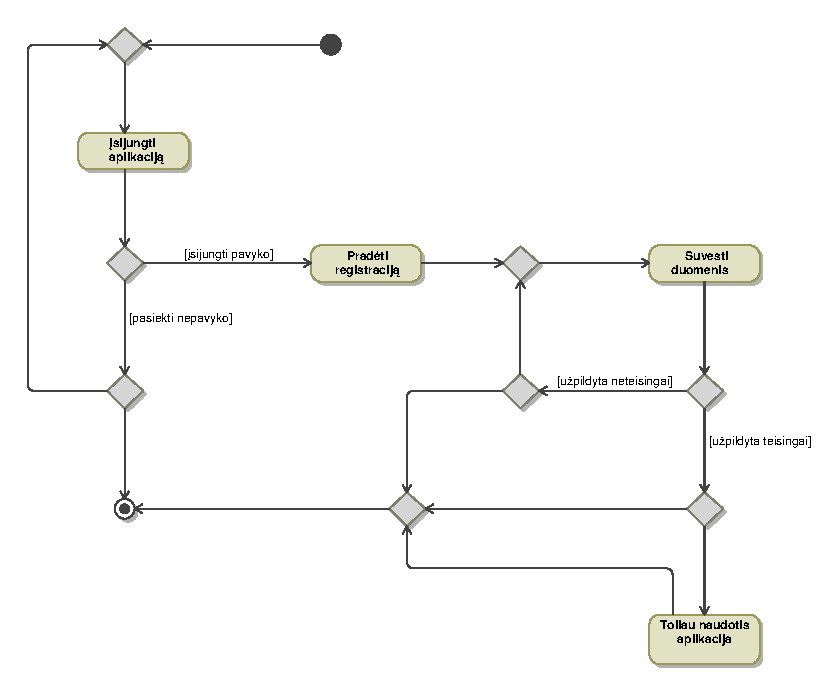
\includegraphics[width=0.9\textwidth]{RegistracijosVeikla.eps}
			\caption{Vartotojo registracijos veiklos diagrama\label{RegisterActivity}}
		\end{center}
	\end{figure}
	
	\pagebreak
	
	\subsection{Skelbimų paieškos veiklos diagrama}
	Procesai, vykstantys skelbimo ieškojimo metu, parodyti \ref{SearchActivity} paveikslėlyje. Pagrindiniame lange vartotojas turi įvesti filtrus, pagal kuriuos bus ieškomi skelbimai. Sistema patikrina, ar įvesti kriterijai yra teisingai suvesti. Jei įvesta klaidingai, vartotojai gali bandyti iš naujo suvesti paieškos kriterijus arba išeiti iš programos. Jei paieškos kriterijai įvesti teisingai, sistema ieško skelbimų. Jei rezultatų nėra, galima pasirinkti kitokius filtrus arba išeiti iš programos. Suradus rezultatų, vartotojas gali pasirinkti skelbimą. Jei jo negalima atidaryti, galima bandyti paiešką atlikti iš naujo. Jei galima atidaryti, vartotojas gali atidaryti skelbimą ir po to grįžti į aplikaciją.
	\begin{figure}[h]
		\begin{center}
			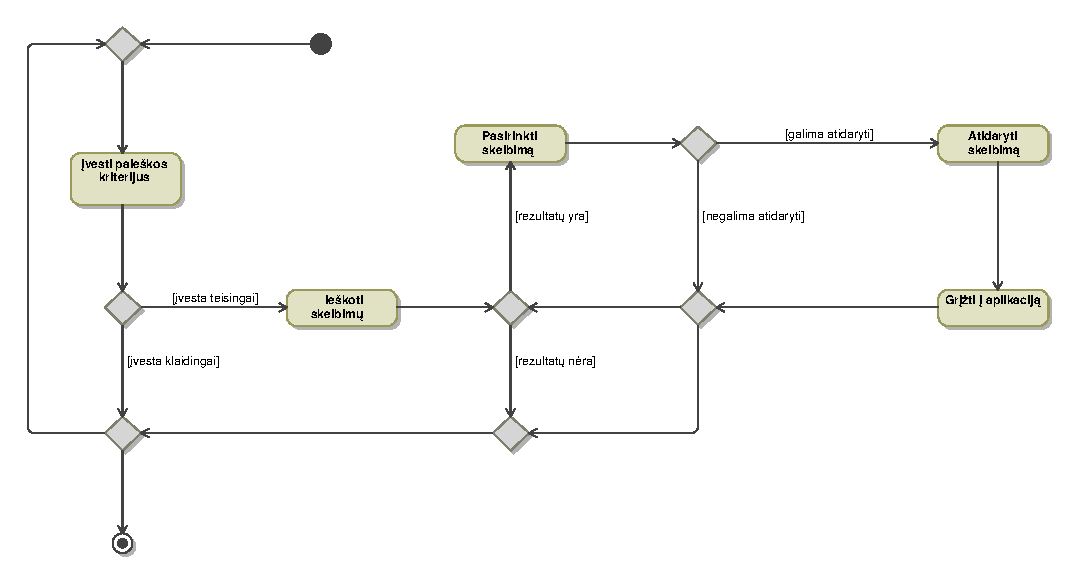
\includegraphics[width=\textwidth]{PaieskosVeikla.eps}
			\caption{Skelbimų paieškos veiklos diagrama\label{SearchActivity}}
		\end{center}
	\end{figure}
	
	\pagebreak
	
	\subsection{Naujo mėgstamo skelbimo veiklos diagrama}
	Procesai, vykstantys vartotojui norint įtraukti skelbimą į mėgstamiausių sąrašą, parodyti \ref{FavActivity} paveikslėlyje. Pirmiausia vartotojas turi prisijungti. Jei to padaryti nepavyksta, jis gali bandyti iš naujo arba išeiti iš programos. Prisijungęs prie sistemos vartotojas ieško jam patinkančio skelbimo ir jį suradęs gali įtraukti į mėgstamiausiųjų sąrašą, o po to ieškoti naujo skelbimo arba išeiti iš šito lango. Jei patinkančio skelbimo vartotojas neranda, tai gali bandyti ieškoti iš naujo arba išeiti iš šito lango.
	\begin{figure}[h]
		\begin{center}
			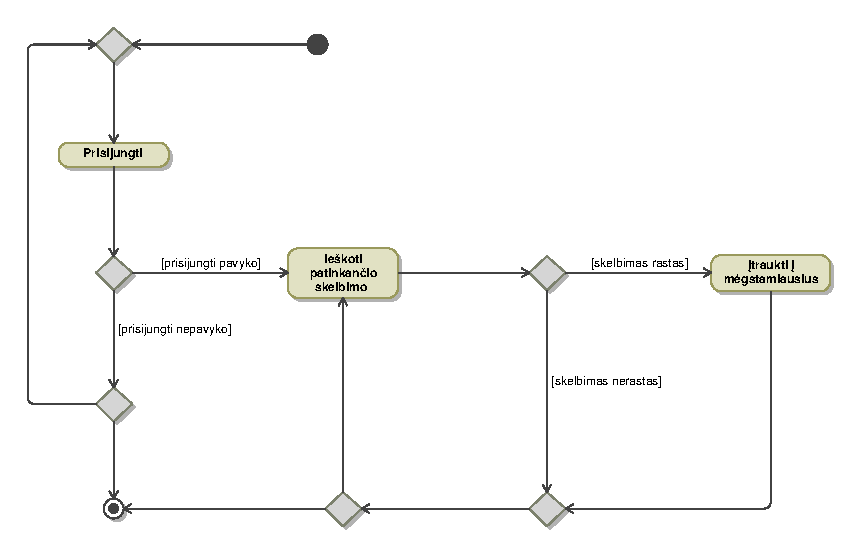
\includegraphics[width=\textwidth]{MegstamiausiuVeikla.eps}
			\caption{Naujo mėgstamo skelbimo veiklos diagrama\label{FavActivity}}
		\end{center}
	\end{figure}
	
	\pagebreak
	
	\section{Komponentų išskirstymas tinkle}
	Šiame skyriuje parodytas sistemos komponentų išdėstymas tinkle.
	\subsection{Komponentų ryšių su artifaktais diagrama}
	
	Žemiau pateiktame komponentų ryšių su artifaktais \ref{ArtComp} paveikslėlyje yra išskirti pagrindiniai sistemos artifaktai. Artifaktus ir komponentus tarpusavyje sieja manifestacijos ryšys. Tai reiškia, kad artifakto sudaromoji dalis yra konkretus komponentas.
	
	\begin{figure}[h]
		\begin{center}
			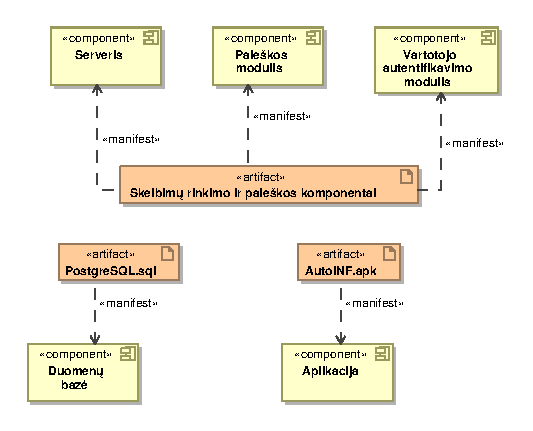
\includegraphics[width=0.8\textwidth]{ArtifaktaiKomponentai.eps}
			\caption{Komponentų ryšių su artifaktais diagrama\label{ArtComp}}
		\end{center}
	\end{figure}

	\begin{indent}
	Sistema susidaro iš trijų pagrindinių dalių - aplikacijos, skelbimų rinkimo ir paieškos komponentų, bei duomenų bazės. Informacijai saugoti apie vartotojų paskyras pasirinkta\break PostgreSQL duomenų bazė.
	\end{indent}
	\pagebreak
	
	\subsection{Diegimo diagrama}
	
	Žemiau pateiktame \ref{Cube} paveikslėlyje yra išskirti fiziniai įrenginiai, rekalingi sistemos darbo palaikymui, bei artifaktų pasiskirstymas tarp jų.\\
	
	\begin{figure}[h]
		\begin{center}
			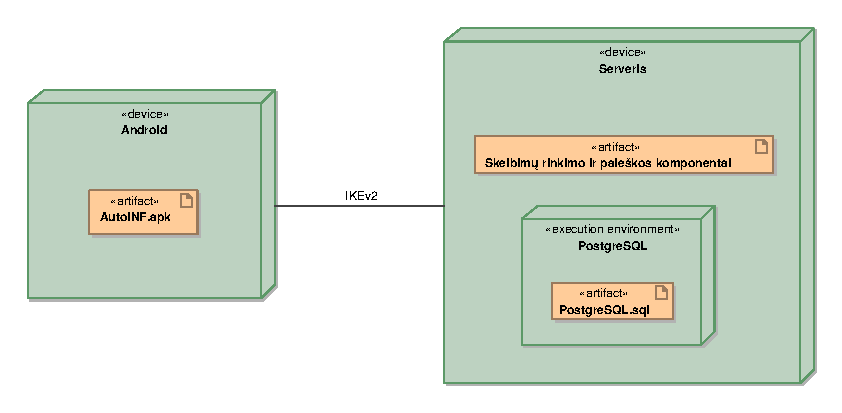
\includegraphics[width=0.9\textwidth]{Mazgai.eps}
			\caption{Diegimo diagrama\label{Cube}}
		\end{center}
	\end{figure}
	
	Beveik visa sistema yra laikoma serveryje. Šiame serveryje yra sudiegiami skelbimų rinkimo ir paieškos komponentai. Tame pačiame serveryje yra ir PostgreSQL duomenų bazė. Vartotojui, norinčiam naudotis sistema iš mobiliojo įrenginio, kuriame yra likusi sistemos dalis, siunčiama užklausa IKEv2 protokolu siekiant gauti sistemos failus.
	\pagebreak
	
	\section*{Rezultatai}
	\addcontentsline{toc}{section}{Rezultatai}
	Šiame laboratoriniame darbe pasitelkiant skirtingus sistemos pjūvius aprašyta knygų dalinimosi sistemos architektūra. Užduočių pjūvyje pasitelkiant užduočių ir sekų diagramomis išaiškinti pagrindiniai agentų (vartotojų ir administratorių) tikslai naudojantis sistema. Loginis pjūvis, pavaizduotas klasių ir objektų diagramomis, leido išskirti pagrindines esybes bei ryšius tarp jų. Kūrimo pjūvyje atlikta sistemos dekompozicija pradedant nuo bendro komponento toliau jį detalizuojant. Procesų pjūvyje, pasitelkiant veiklos diagramas, išskirti procesai, jų komunikacija, objektų gyvavimo ciklai. Galiausiai fiziniame pjūvyje apibrėžtas sistemos išdėstymas tinkle. Šis skirtingų požiūrių rinkinys leido aptikti ankčiau sukurtame sistemos prototipe buvusias klaidas bei išplėtoti tinkamą sistemos architektūrą.
	\pagebreak

	\section*{Išvados}
	\addcontentsline{toc}{section}{Išvados}
	Remiantis rezultatais bus galima sukurti mobiliesiems įrenginiams skirtą programėlę, kuri leis vienoje vietoje pasiekti automobilių skelbimus iš visos Europos, taip palengvindama paieškos procesą daugeliui žmonių. 
	\pagebreak

	\section*{Terminų žodynas}
	\addcontentsline{toc}{section}{Terminų žodynas}	
	
	\bigskip
	\textbf{Vartotojas} - žmogus, besinaudojantis sistema.
	
	\textbf{Administratorius} - vartotojas, kuriam suteikiamos teisės tvarkyti šaltinius.
	
	\textbf{Skelbimas} - iš skelbimų šaltinio gautas sistemoje patalpintas skelbimas.
	
	\textbf{Šaltinis} - internetinis skelbimų puslapis, iš kurio gaunami skelbimai naudojami sistemoje.
	
	\textbf{Megstamas / mėgstamiausias} - skelbimas, kurį vartotojas išsaugo galimam lengvam ir greitam vėlesniam pasiekiamumui.
	\pagebreak

	\section*{Literatūros sąrašas}
	\addcontentsline{toc}{section}{Literatūros sąrašas}	
	
	Doug Rosenberg and Matt Stephens „Use Case Driven Object Modeling with UML“
\end{document}